\documentclass[10pt]{beamer}
\setbeamertemplate{navigation symbols}{\insertlogo}

%\documentclass[handout,dvips,11pt,grey]{beamer}

%\usetheme{Goettingen}
%\usetheme{Warsaw}
\usetheme{Hannover}

%\usepackage{tikz,pgf}
\usepackage{multicol}
\usepackage{amsmath,amsthm,amssymb}
%\usepackage{epstopdf}
%\usepackage{xspace}
\usepackage{wrapfig}

\usepackage{verbatim}
%\usepackage{circuitikz}
%\usepackage{graphicx}
\usepackage{comment}
%\usepackage{array}
\usepackage{coffee4}

\title{Identifying Subject Matter Experts}
\subtitle{Extending Author Topic Modeling}
\author{Philip Robinson}
\date{\today}
\institute{Presented to 5x \\ NASA - Jet Propulsion Lab}

\DeclareMathOperator*{\argsort}{argsort}

  \logo{
\includegraphics[height=.7cm]{./logo.png}}


\begin{document}

\begin{frame}
  \titlepage


\end{frame}

\section{Introduction}
\begin{frame}{Introduction - Philip Robinson}
  {\bf Computer Science MSc at Oregon Health and Science}

  \vspace{1em}

  {\em Thanks to my mentor Ian Colwell, from the OCIO (1762)}

  \begin{multicols}{2}
    
\includegraphics[width=\columnwidth]{./philip.jpg}

    \begin{itemize}
    \item probabilistic programming
    \item language processing
    \item image processing
    \item audio processing
    \item stem education
    \item environmental sciences
    \item[$\star$] information retrieval
    \end{itemize}

  \end{multicols}

\end{frame}

\begin{frame}{Presentation Overview}
  \tableofcontents

\end{frame}



\section{Problem Description}

\begin{frame}{Problem Description}
  Our customers, Office of Safety and Mission Success (5x), are interested in
  identifying experts for resolving anomaly reports in the Problem Reporting System (PRS)

  \vspace{2em}

  % meditate on including prior work
  OCIO (17x) has been previously asked for subject matter expert
  identification systems and document similarity tools, so show
  particular interest is solutions that provide similarity metrics
  and can generalize to other teams and corpora.


  \begin{itemize}
  \item A-Team heirarchical frequent item set expert exploration tool
  \item TechConnect self reported skills host
  \item Gateway Profiles
  \end{itemize}
\end{frame}

\begin{frame}{Motivating Story}
  \begin{itemize}
  \item Domain experts are lost between projects
  \item Domain experts are often coupled to a single project
  \item Very few candidates resolve the majority of tickets
  \end{itemize}

    \begin{itemize}
  \item Expert discoverability
  \item Load balancing employees
  \item Identification of knowledge gaps
  \end{itemize}


\end{frame}

\begin{frame}{Objective}
  \begin{itemize}
  \item Assign \& Resolve anomalies quicker
  \item Support expert discovery
  \item Find employees with similar domain expertise
    %\item Identify knowledge gaps against a corpus
  \end{itemize}
\end{frame}


\begin{frame}{Data Provided for Internship}
  \begin{itemize}
  \item Problem Reporting System (Anomalies)
    \begin{itemize}
    \item Problem Failure Report (PFR)
    \item Developmental Problem Failure Report (DPFR)
    \item Incident Surprise Anomaly (ISA)
    \end{itemize}
  \end{itemize}

\end{frame}


%\begin{frame}{Terms}
%\end{frame}

\section{Proposed Approach}

\begin{frame}{Approach}
  {\bf Author-Topic-Modeling}

% Fitting authorship as a generative model allows us to mathematically abstract and describe a provided corpus, allowing us to ask deeper questions about incoming documents. We elect using the Author-Topic-Model (ATM) to ask the `most likely author' of a document, as a proxy for expertise.

  \begin{multicols}{2}

  \begin{itemize}
  \item Interpret doc as Bag-of-Words\footnote{equivelent to multinomial over vocabulary}
  \item Model/Fit topics as mixture of words
  \item Author \& document are projected into topic-space
  \item Measure distance from author to document
  \end{itemize}

  \begin{figure}
  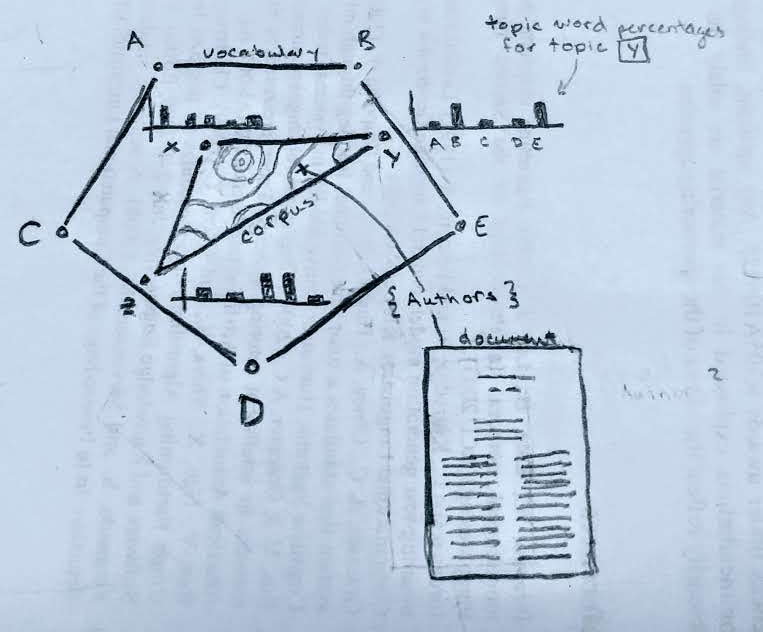
\includegraphics[width=\columnwidth]{./lda-draw.jpg}
  \caption{Latent Dirichlet Allocation}
  \end{figure}

  \end{multicols}

  \vspace{-2em}
  \begin{align*}
    T(x) &= \texttt{Project $x$ into topic-space} \\
    R_d &= \argsort_{a\in A} \left\{Distance(T(a),T(d))\right\}
  \end{align*}

\end{frame}


\section{Results}

\begin{frame}{Ranking}

  Given Authors/Experts in a ``Topic Space'' and a mapping from document to ``Topic Space'', we can rank experts for a document. % Ideally this is done with the probability of an author given a document, but presently we use distribution similarity metrics to rank authors.

  \begin{multicols}{2}
    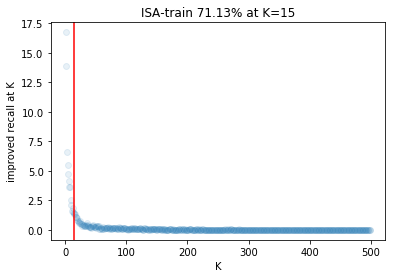
\includegraphics[width=\columnwidth]{./recall-train-isa.png}

    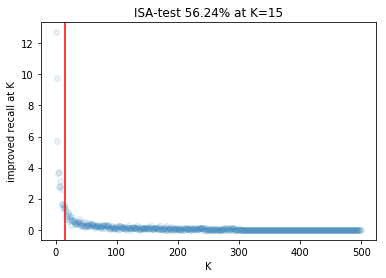
\includegraphics[width=\columnwidth]{./recall-test-isa.png}
  \end{multicols}

  K is cutoff for suggested candidates
\end{frame}

\begin{frame}{Recieving Candidates}
  {\bf Results begin at 4 words}

  It is possible to get interesting results at a document length of 4 words,
  however it is hard to know why these results are interesting.
  This is an example of directly searching for experts.

  \begin{multicols}{2}
    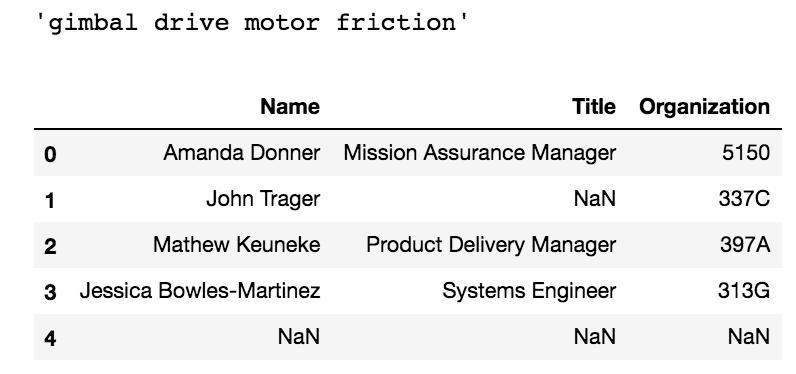
\includegraphics[width=\columnwidth]{query1.png}

    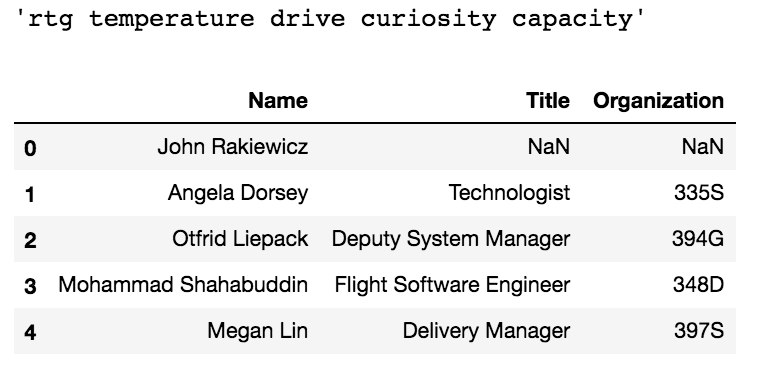
\includegraphics[width=\columnwidth]{query2.png}
  \end{multicols}

%  Documents queries generate better results. These examples are
%  currently unable to demo.

\end{frame}


\begin{frame}{How does word count effect recall?}
  {\bf Best results at 30 words}

  We are interested in understanding how much text is required to inform
  our model prediction. For these plots, we randomly subset texts for
  known ticket-expert pairs and observe the expert's new ranking.

  \begin{multicols}{2}
    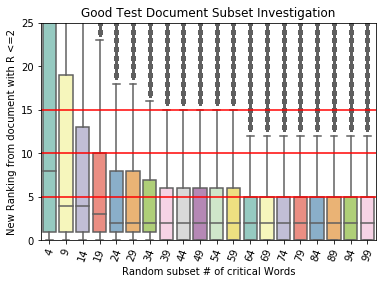
\includegraphics[width=\columnwidth]{low-ranked-downsample.png}
    Expert found in top 2\\
    24 critical words

    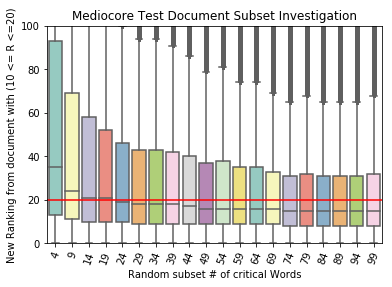
\includegraphics[width=\columnwidth]{mid-ranked-downsample.png}
    expert found in 10-20 range\\
    29 critical words
  \end{multicols}
\end{frame}

\begin{frame}{Number of Publications}
  These plots show the ranking of True authors, against a provided document. The \texttt{x-axis} tells us how many publications were attributed to an author, the \texttt{y-axis} tells us what rank they received when evaluated against the specific document. The darkness of a hexblock indicates the population density of an \texttt{(X,Y)} location, like a heatmap.

  \begin{multicols}{2}
    Train
    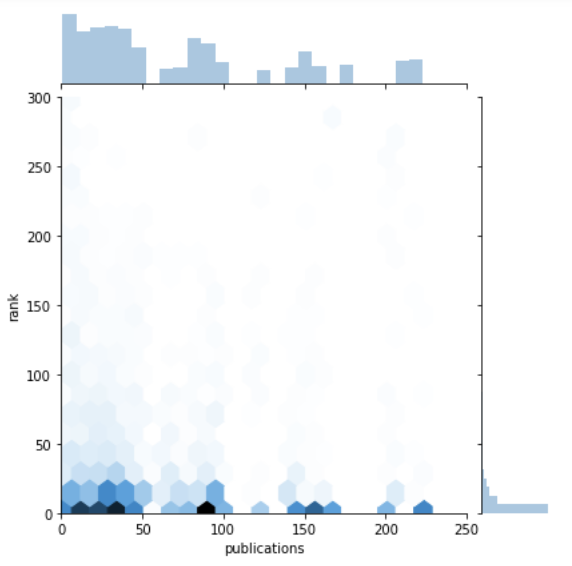
\includegraphics[width=.9\columnwidth]{./Train.png}

    Test
  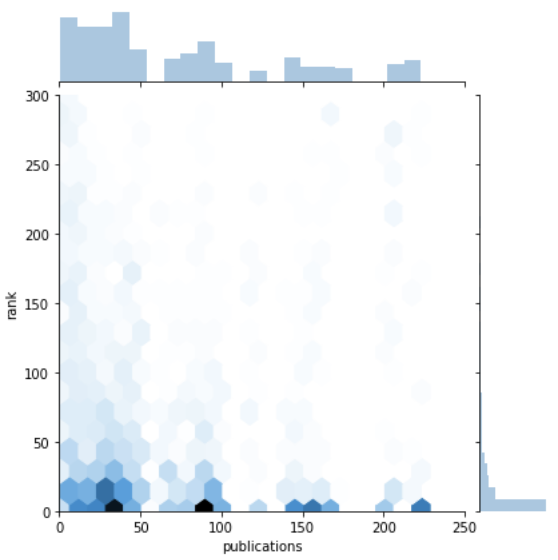
\includegraphics[width=.9\columnwidth]{./Test.png}
  \end{multicols}{2}
\end{frame}

\begin{frame}{Malicious Candidates}
  \begin{itemize}
  \item Over represented Authors (becomes hyperparameter)
  \item Non-experts associated tickets
  \end{itemize}

  \begin{quote}
    Over represented candidates appear more as generalists, and float to the top of our recomendations list. Currently we bound attribution counts.
  \end{quote}
\end{frame}

\section{Conclusion}

\begin{frame}{Presentations}
  \begin{itemize}
  \item Internship presentations
  \item Use of Topic Modeling - itds \& search team
  \item Topic modeling for non-statisticians - opslab
  \item Customer presentation - 5x
  \end{itemize}
\end{frame}

\begin{frame}{What we have}
  \begin{multicols}{2}
  \begin{itemize}
  \item Generalized
    \begin{itemize}
    \item preprocessing
    \item hyperparameter election
    \item model biulding
    \item API access
    \end{itemize}
  \item \hyperlink{file:///Users/philipr/git/jpl-playground/code/site/index.html}{Web Interface}
  \end{itemize}

  \columnbreak

  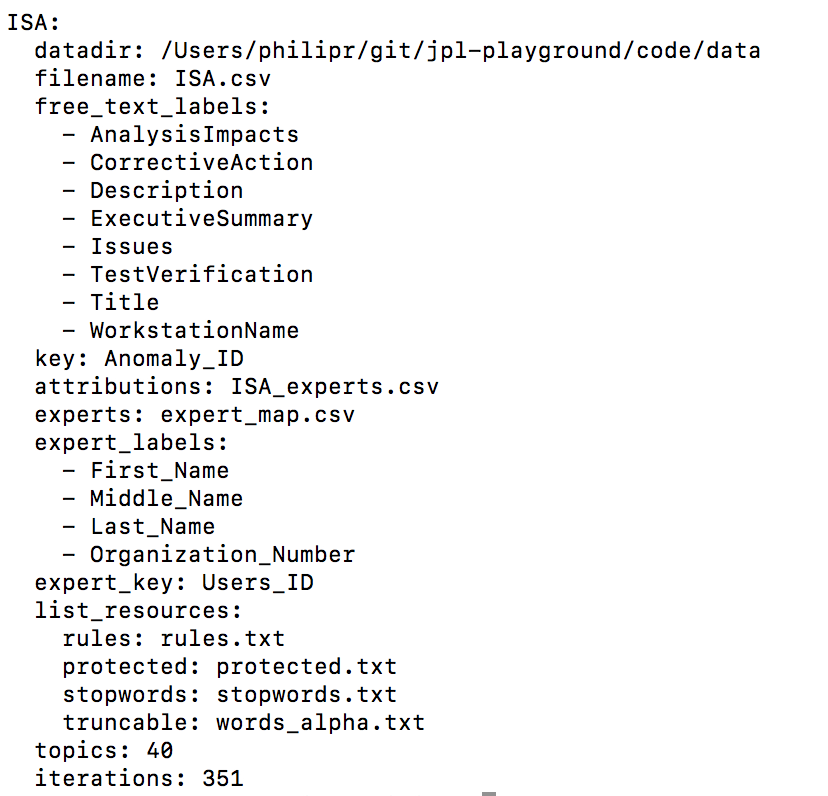
\includegraphics[width=\columnwidth]{./config.png}
  \end{multicols}
\end{frame}

\begin{comment}
\begin{frame}{Thanks}
  I received a lot of input in for this project from my team.
  Their insight, especially, bridged the gap from academic to practical evaluation of models,
  and I sincerely appreciate their contributions.

  \begin{itemize}
  \item Ian Colwell
  \item Valentinos Constantinou
  \item Jerry Chen
  \item Leslie Callum
  \item Bruce Waggoner
  \item Harald Schone
  \item Chris Mattmann
  \item[] et. al.
  \end{itemize}

\end{frame}
\end{comment}

\begin{frame}{Internship Notes}

%  I had never implemented a recommender system, nor used topic modeling in
%  a project prior to this task. I will be leaving JPL with a holistic understanding
%  of topic modeling, and a much better understanding of recommender systems.

\vspace{1em}

%  This work has encouraged me to look at continued employment in applications of
%  machine learning for information retrieval more realistically. I'm also interested
%  in keeping in touch over future employment opportunities with JPL.

  \vspace{1em}

  Having multiple interns work with the same data helps. We were able to work through
  data difficulties together, and share results.
\end{frame}


\begin{frame}{Thanks}

  I received a lot of input in for this project from my team.
  Their insight, especially, bridged the gap from academic to practical evaluation of models,
  and I sincerely appreciate their contributions.

  \begin{itemize}
  \item Ian Colwell
  \item Valentinos Constantinou
  \item Jerry Chen
  \item Leslie Callum
  \item Bruce Waggoner
  \item Harald Schone
  \item Chris Mattmann
  \item[] et. al.
  \end{itemize}


\end{frame}

\end{document}
